\chapter{RESULT ANALYSIS}
\label{anotherchapter}
\vspace{-3em}

This chapter provides a detailed discussion of the findings and analysis .....

 \section{Evaluation Metrics}
    Evaluation metrics are measures used to assess the performance of machine learning models. The values of these metrics tell how well a model is performing. Evaluation metrics are essential for comparing different models or tuning their parameters.

 \subsection{Accuracy}
 Accuracy measures the proportion of correctly classified data out of the total number of data. It is the ratio of the number of correct predictions to the total number of predictions made by the model. 
 \begin{equation}
\text{Accuracy} = \frac{\text{True Positives + True Negatives}}{\text{Total Predictions}}
\end{equation}

\subsection{Precision}
Precision is a metric that measures the number of true positive predictions out of all positive predictions made by the model. It is the ratio of true positives to the sum of true positives and false positives. 
\begin{equation}
\text{Precision} = \frac{\text{True Positives}}{\text{True Positives + False Positives}}
\end{equation}



\subsection{Dice Coefficient}
The Dice coefficient is a metric used to evaluate the similarity or overlap between two sets. In the context of image segmentation, it measures the agreement between the predicted segmentation mask and the ground truth mask. The Dice coefficient ranges from 0 to 1, with higher values indicating greater overlap between the predicted and ground truth masks. 

\begin{equation}
\text{Dice Coefficient} = 2 \times \frac{\text{Precision} \times \text{Recall}}{\text{Precision + Recall}}
\end{equation}

   

\subsection{Mean Absolute Error (MAE)}
Mean Absolute Error (MAE) is a metric used to measure the average magnitude of errors between predicted and actual values in regression tasks. It is the average of the absolute differences between predicted and actual values. MAE provides a straightforward interpretation of prediction accuracy with lower values indicating better performance.
\begin{equation}
\text{MAE} = \frac{1}{n} \sum_{i=1}^{n} |y_i - \hat{y}_i|
\end{equation}
where $y_i$ represents the true values, $\hat{y}_i$ represents the predicted values, and $n$ represents the total number of samples.

\subsection{Mean Square Error (MSE)}
Mean Square Error (MSE) is a metric used to measure the average squared differences between predicted and actual values in regression tasks. It is the average of the squared differences between predicted and actual values. MSE penalizes larger errors more heavily than MAE which makes it sensitive to outliers in the data.

\begin{equation}
\text{MSE} = \frac{1}{n} \sum_{i=1}^{n} (y_i - \hat{y}_i)^2
\end{equation}
where $y_i$ represents the true values, $\hat{y}_i$ represents the predicted values, and $n$ represents the total number of samples.
\subsection{Root Mean Square Error (RMSE)}
Root Mean Squared Error (RMSE) is a measure used to quantify the average difference between predicted values and actual values in a dataset. RMSE is a popular metric in fields like statistics and machine learning, helping to measure how close predictions are to the actual values in a simple and understandable way.
\begin{equation}
\text{RMSE} = \sqrt{\frac{1}{n} \sum_{i=1}^{n} (y_i - \hat{y}_i)^2}
\end{equation}
where $y_i$ represents the true values, $\hat{y}_i$ represents the predicted values, and $n$ represents the total number of samples.


\section{Result and Performance Analysis for Green Space Detection}

\begin{table*}[h]
\centering
\caption{Performance Comparison of Various Segmentation Models on Pre-Existing and Custom Dataset}
\label{tab2}
\small % Reduce font size
%\def\arraystretch{0.9}
%\resizebox{\textwidth}{!}{
\begin{tabular}{p{.13\linewidth}p{.12\linewidth}p{.12\linewidth}p{.11\linewidth}p{.12\linewidth}p{.12\linewidth}p{.11\linewidth}}
    \hline
    \textbf{ }&
    \multicolumn{3}{l}{Pre-existing Dataset} & \multicolumn{3}{l}{Custom Dataset}\\
    \cline{1-7}
    Category & Accuracy & Precision & Dice Coefficient  & Accuracy & Precision & Dice Coefficient  \\
    
    \hline
    UNet    
     & \textbf{0.92}
     & 0.83
     & 0.69
     & \textbf{0.89}
     &  \textbf{0.87}
     & \textbf{0.73}    
\\
%\hline
Segnet
     & 0.88
     & \textbf{0.86}
     &  \textbf{0.77}
     &  0.84
     &  0.73
     &  0.60   
\\
%\hline
DeepLabV3+
     & 0.78
     & 0.78
     & 0.65
     &  0.87
     &  0.76
     &  0.71  
\\
\hline
\end{tabular}
\end{table*}


%In Figure \ref{fig3}, an input image is taken from the pre-existing dataset and it's corresponding binary mask which has been used as ground truth. The resultant segmented images from various trained models have been displayed. Similarly, in Figure \ref{fig4}, an input image is taken from the custom dataset and it's corresponding binary mask which has been used as ground truth. The resultant segmented images from various trained models have been displayed.

\subsection{Comparison with Pre-existing and Custom dataset}
Table \ref{tab2} shows the results for the performance comparison of the three state-of-the-art models on the entire pre-existing and custom dataset. It is seen from the table that, for the pre-existing dataset, U-Net is giving the highest accuracy but Segnet has the highest precision and dice-coefficient. On the other hand, for the entire custom dataset, UNet gives the highest accuracy, precision and dice coefficient.

\begin{table}[!htbp]
\centering
\caption{Performance Analysis of Various Segmentation Models on Custom Dataset Categories}
\label{tab3}
\renewcommand{\arraystretch}{1.5} % Adjust vertical spacing
\small % Reduce font size
\begin{tabular}{p{.13\linewidth}p{.07\linewidth}p{.07\linewidth}p{.07\linewidth}p{.07\linewidth}p{.07\linewidth}p{.07\linewidth}p{.07\linewidth}p{.07\linewidth}p{.07\linewidth}}
    \hline
    Category &
    \multicolumn{3}{l}{Park} & \multicolumn{3}{l}{Forest} & \multicolumn{3}{l}{Residence}\\
    \cline{1-10}
    Model & Accuracy & Precision & Dice Coefficient & Accuracy & Precision & Dice Coefficient & Accuracy & Precision & Dice Coefficient\\
    \hline
    UNet    
     & \textbf{0.87}
     & \textbf{0.85}
     & \textbf{0.72}
     & \textbf{0.88}
     & \textbf{0.82}
     & \textbf{0.77}
     & \textbf{0.88}
     & \textbf{0.86}
     & \textbf{0.71}     
\\
%\hline
Segnet
     & 0.74
     & 0.51
     & 0.59
     & 0.71
     & 0.48
     &  0.37
     & 0.81
     & 0.67
     & 0.56    
\\
%\hline
DeepLabV3+
     & 0.83
     &  0.77
     & 0.58
     & 0.73
     & 0.43
     & 0.42
     & 0.86
     & 0.72
     & 0.67     
\\
\hline
\end{tabular}

\label{table3}
\end{table}


The custom dataset has been further broken down and the results for each category are shown in Table \ref{tab3}. For all three categories, U-Net is seen to give the highest accuracy, precision and dice coefficient. Another noteworthy observation is that for the Forest dataset, precision, and dice coefficient are significantly low for Segnet and DeepLabV3+ models as the forest dataset contains a much lower number of images among all the categories. 

Although U-Net exhibited higher accuracy, Segnet is superior in both precision and dice-coefficient, portraying its ability to precisely identify as well as outline the area of interest through better localization. Thus, from the table and figures, it is evident that for the pre-existing dataset, Segnet outperforms the other two models while for the custom dataset, U-Net performs the best.

\begin{figure*}[!htbp]
\centering
 
    \begin{subfigure}[t]{0.18\textwidth}
        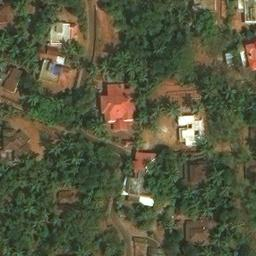
\includegraphics[width=\linewidth]{figures/inputkaggle.jpg}
        \caption{Original Image from Pre-existing Dataset}
    \end{subfigure}
    \hfill
    \begin{subfigure}[t]{0.18\textwidth}
        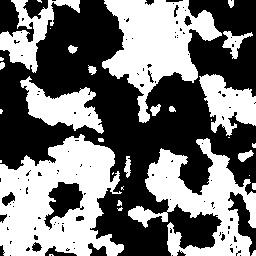
\includegraphics[width=\linewidth]{figures/maskkaggle.jpg}
        \caption{Ground Truth Mask}
    \end{subfigure}
    \hfill
    \begin{subfigure}[t]{0.18\textwidth}
        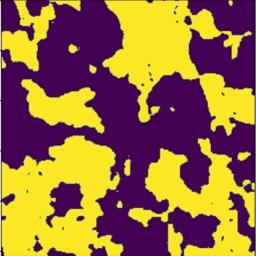
\includegraphics[width=\linewidth]{figures/unetkaggle.jpg}
        \caption{Segmentation using U-Net}
    \end{subfigure}
    \hfill
    \begin{subfigure}[t]{0.18\textwidth}
        \includegraphics[width=\linewidth]{figures/dlV3kaggle.jpg}
        \caption{Segmentation using DeepLabV3}
    \end{subfigure}
    \hfill
    \begin{subfigure}[t]{0.18\textwidth}
        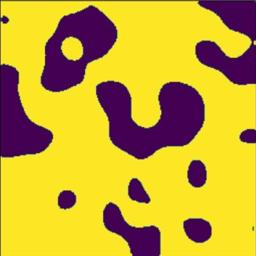
\includegraphics[width=\linewidth]{figures/segnetkaggle(0.5 threshold).jpg}
        \caption{Segmentation using SegNet}
    \end{subfigure}
    \caption{Outputs from Different Models for Pre-existing Dataset}
    \label{fig3}
   
\end{figure*}
\begin{figure*}[!htbp]
\centering
    \begin{subfigure}[t]{0.18\textwidth}
        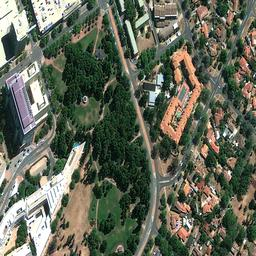
\includegraphics[width=\linewidth]{figures/input custom.jpg}
        \caption{Original Image from Custom Dataset}
    \end{subfigure}
    \hfill
    \begin{subfigure}[t]{0.18\textwidth}
        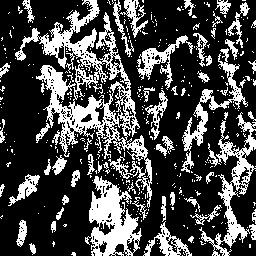
\includegraphics[width=\linewidth]{figures/maskcustom.jpg}
        \caption{Ground Truth Mask}
    \end{subfigure}
    \hfill
    \begin{subfigure}[t]{0.18\textwidth}
        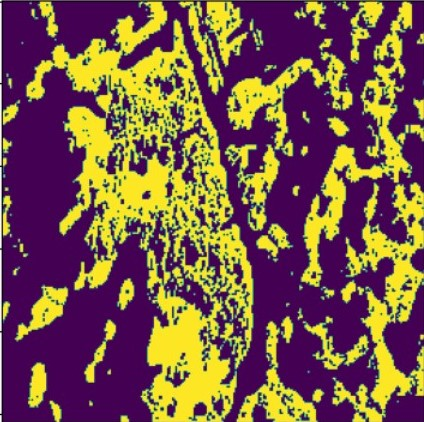
\includegraphics[width=\linewidth]{figures/unetcustom.jpg}
        \caption{Segmentation using UNet}
    \end{subfigure}
    \hfill
    \begin{subfigure}[t]{0.18\textwidth}
        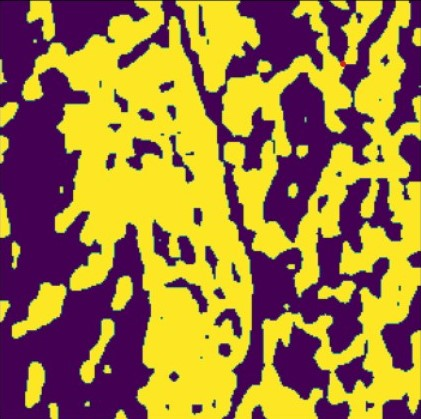
\includegraphics[width=\linewidth]{figures/dlv3custom.jpg}
        \caption{Segmentation using DeepLabV3}
    \end{subfigure}
    \hfill
    \begin{subfigure}[t]{0.18\textwidth}
        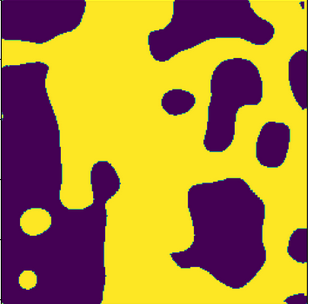
\includegraphics[width=\linewidth]{figures/segnetcustom(0.5).png}
        \caption{Segmentation using SegNet}
    \end{subfigure}
    \caption{Outputs from Different Models for Custom Dataset}
    \label{fig4}
\end{figure*}


\subsection{Comparative Analysis of Ensemble Learning Techniques}

\begin{comment}
   \begin{longtable}{l p{2cm} p{1.8cm} p{1.8cm} p{1.8cm} p{1.8cm} p{1.8cm}}
    \caption{Performance Analysis of Ensemble Learning on Pre-Existing and Custom Datasets} \label{table4} \\
    
    \hline
     & \multicolumn{3}{c}{\textbf{Pre-Existing Dataset}} & \multicolumn{3}{c}{\textbf{Custom Dataset}} \\
    \hline
     \textbf{Combination}& \textbf{Accuracy} & \textbf{Precision} & \textbf{Dice-Coefficient} & \textbf{Accuracy} & \textbf{Precision} & \textbf{Dice-Coefficient} \\
    \hline
    \endfirsthead
    
    \multicolumn{7}{c}{{\tablename} \thetable{} -- Continued from previous page} \\
    \hline
     & \multicolumn{3}{c}{\textbf{Pre-Existing Dataset}} & \multicolumn{3}{c}{\textbf{Custom Dataset}} \\
    \hline
     \textbf{Combination}& \textbf{Accuracy} & \textbf{Precision} & \textbf{Dice-Coefficient} & \textbf{Accuracy} & \textbf{Precision} & \textbf{Dice-Coefficient} \\
    \hline
    \endhead
    
    UNet and Segnet & 0.83 & 0.87 & 0.88 & 0.80 & 0.72 & 0.68\\ \hline
    UNet and DeepLabV3+ & 0.25 & 0.35 & 0.50 & 0.83 & 0.88 & 0.57 \\ \hline
    DeepLabV3+ and Segnet & 0.65 & 0.93 & \textbf{0.91} & 0.81 & 0.95 & 0.77 \\ \hline
    UNet, Segnet and DeepLabV3+& \textbf{0.84} & \textbf{0.96} & 0.82 & \textbf{0.94} & \textbf{0.96} & \textbf{0.91} \\
    
    \hline
\end{longtable} 
\end{comment}


\begin{table*}[htbp]
    \centering
    \caption{Performance Analysis of Ensemble Learning on Pre-Existing and Custom Datasets}
    
    \begin{tabular}{p{.14\linewidth}p{.12\linewidth}p{.12\linewidth}p{.11\linewidth}p{.12\linewidth}p{.12\linewidth}p{.11\linewidth}}
    \hline
    \textbf{ }&
    \multicolumn{3}{l}{Pre-existing Dataset} & \multicolumn{3}{l}{Custom Dataset}\\
    \cline{1-7}
    Combination & Accuracy & Precision & Dice Coefficient  & Accuracy & Precision & Dice Coefficient  \\
        \hline
        UNet,Segnet & 0.83 & 0.87 & 0.88 & 0.80 & 0.72 & 0.68\\% \hline
        UNet, DeepLabV3+ & 0.25 & 0.35 & 0.50 & 0.83 & 0.88 & 0.57 \\ %\hline
        DeepLabV3+, Segnet & 0.65 & 0.93 & \textbf{0.91} & 0.81 & 0.95 & 0.77 \\ %\hline
        UNet, Segnet and DeepLabV3+& \textbf{0.84} & \textbf{0.96} & 0.82 & \textbf{0.94} & \textbf{0.96} & \textbf{0.91} \\
        \hline
    \end{tabular}
    
    \label{table4}
\end{table*}


Table \ref{table4} shows the Accuracy, Precision, and Dice-Coefficient for all possible combinations of the deep learning models, that is ensemble learning. In the Preexisting dataset section of table \ref{table4}, all the combination demonstrates the varying level of accuracy, precision, and dice coefficient for the collected data set with combination 4 (UNet-Segnet-DeepLabV3+) having the highest accuracy (0.84) and precision (0.96) among all the combinations. However, combination 3 (DeepLabV3+-Segnet) shows the highest dice-coefficient of 0.91 which is slightly more than the dice-coefficient of combination 4 (UNet-Segnet-DeepLabV3+). It is also evident that the performance of combination 2 (UNet-DeepLabV3+) has a significant discrepancy from the other combinations.
\\The custom dataset section of table \ref{table4} exhibits that combination 4 \\(UNet-Segnet-DeepLabV3+) has the highest accuracy (0.94) along with the highest precision (0.96) and dice coefficient (0.91). Additionally, it is observed that the performance of dice-coefficient of the models for the custom dataset is notably below standard compared to the pre-existing dataset.%\subsection{Comparative Analysis}
%This section compares the performance metrics of the applied machine learning models using the aforementioned datasets as described earlier in 
\\\\From Tables \ref{tab2} and \ref{table4}, it is visible that SegNet excels in accuracy for the pre-existing dataset, while a combination of SegNet, UNet, and DeepLabV3+ performs best for the custom dataset. In terms of precision, the combination of SegNet, UNet, and DeepLabV3+ outperforms others on both datasets. For dice-coefficient, the combination of UNet and SegNet is best for the pre-existing dataset, and SegNet, UNet, and DeepLabV3+ excel for the custom dataset. In conclusion, the ensemble learning technique executes better than the deep learning techniques and the combination of SegNet, UNet and DeepLabV3 on custom dataset gives the most desirable result. Therefore it is proposed as the best model for segmenting green space from aerial images.  

\subsection{K-fold Cross-Validation}

\begin{table}[!h]
    \centering
    \caption{5-fold Cross Validation Results}
    \begin{tabular}{l p{2cm} p{2cm} p{3cm}}
        \hline
        Test Set & Accuracy & Precision & Dice Coefficient \\
        \hline
        1 & 0.95 & 0.95 & 0.91  \\
        2 & 0.94& 0.95 & 0.91 \\ 
        3 & 0.95& 0.96& 0.92\\ 
        4 & 0.94& 0.96& 0.92\\ 
        5 & 0.94& 0.96& 0.92\\ 
        \textbf{Average} & \textbf{0.94} & \textbf{0.96} & \textbf{0.92} \\
        \hline
    \end{tabular}
    \label{table6}
\end{table}


\section{Result and Performance Analysis of Green Space Prediction}


\subsection{Comparative Analysis of RNN Models}


\begin{longtable}{@{}lccc@{}}
\label{RNN_model}
    \caption{Test Metrics for Different RNN Models} \\
    \hline
    Model & Test MAE & Test MSE & Test RMSE \\
    \hline
    \endfirsthead
    
    \multicolumn{4}{c}{{\tablename} \thetable{} -- Continued from previous page} \\
    \hline
    \textbf{Model} & \textbf{Test MAE} & \textbf{Test MSE} & \textbf{Test RMSE} \\
    \hline
    \endhead
    
    GRU & 0.7741 & 0.9600 & 0.9798 \\
    LSTM & \textbf{0.5764} & \textbf{0.6216} & \textbf{0.7884} \\
    ATT-LSTM & 1.600 & 5.0211 & 2.2408 \\
    ATT-GRU & 1.888 & 5.586 & 2.3635 \\
    \hline
\end{longtable}

Table \ref{RNN_model} portrays the evaluation results of the four RNN models performed. With a Test MAE of 0.7741, MSE of 0.9600 and an RMSE value of 0.9798, the GRU model showed a moderate performance and provided reasonable predictions. However, there is room for improvement in terms of minimizing errors. On the contrary, both Attention-based LSTM and Attention-based GRU exhibit higher error metrics compared to their basic architectures. Therefore, the application of attention mechanisms to the RNN architectures may not be the best choice for the required task. It is visible that the LSTM model outperforms the other models, achieving the lowest values across all three evaluation metrics.  Thus, LSTM is proposed as the most fitting RNN model for predicting change in GVI for a selected location. 


\section{Experimental Evaluation}
To evaluate the effectiveness of the proposed framework, historical images from 2000 to 2015 were used to forecast the same location's change in green space over the next five years. Thus, the GVI change from 2015 to 2020 was predicted using segmented photos of the same locations from 2000, 2005, 2010, and 2015. This range of years was selected as it is not possible to calculate the ground truth value of years after 2024. In addition, images prior to 2000 are not easily accessible. Therefore, in this experiment,  2015 has been considered as the current year and 2020 will be the future year following a five-year gap. The procedure followed and the results achieved from the experiment are presented in this section.
\subsection{Experimental Procedure}
The custom dataset was split into 80\% train data and 20\% test data. As the dataset contains segmented images from 4 different years with a five-year gap, the number of pairs created was 3, which are as follows:
\begin{itemize}
  \item $Pair_1$: \{$Image_{2000}$, $Image_{2005}$\}
  \item $Pair_2$: \{$Image_{2005}$, $Image_{2010}$\}
  \item $Pair_3$: \{$Image_{2010}$, $Image_{2015}$\}
  \end{itemize}
  Each pair of test data was sent to a separate siamese model \{$S_1$, $S_2$, $S_3$\}, which was previously trained using segmented pictures from the chosen years. This is module 1 of the proposed framework. The exact siamese models trained earlier for $Pair_1$, $Pair_2$ and $Pair_3$ in Chapter 3 have been used in this experiment.  From the Siamese models, the GVI difference value between the paired images $\{\Delta\text{GVI}_{\text{P}_1\\}, \Delta\text{GVI}_{\text{P}_2},
\Delta\text{GVI}_{\text{P}_{3}}\}$ were obtained were then fed to the  LSTM model. This is the module 2 of the proposed framework. Finally, the LSTM model gives a value as output which is the GVI difference between the latest year (2015) and the next 5 years (2020). The predicted GVI differences were then compared with ground truth values and metrics such as MAE, MSE, and RMSE were calculated. 
\subsection{Experimental Result }

After experimenting as described in 4.4.1, an MAE of 0.2707, MSE of 0.1492, and an RMSE of 0.3862 was achieved. These results imply that the proposed framework, utilizing a combination of multiple Siamese neural networks and an LSTM model, performs reasonably well in forecasting the changes in green space. The low error metrics demonstrate the acquired precision and accuracy and highlight the model's capability to offer predictions about future changes in the GVI value of a given location.

